\chapter{Gaussian elimination and quantum observables}
\label{chap:gaussian-observables}

The transfer in Chapter~\ref{chap:higher-associativity} starts with a
differential satisfying the graded Leibniz rule.
Eliminating a variable changes the relations between its polynomial
observables. A quadratic action produces a complex in which the variable
represents zero and its square represents a nonzero scalar.
A second-order term in the differential accounts for this failure of
polynomial multiplication on cohomology.

\section{The one-variable Gaussian complex}
\label{sec:gaussian-one-variable}

\subsection{The real Gaussian average}

For a real variable $x$, the quadratic action
\[
 S(x)=\frac{x^2}{2}
\]
has its minimum at zero. Fix a positive real number $h$, and associate
to $x$ the weight
\[
 w_h(x)=\exp\!\left(-\frac{x^2}{2h}\right).
\]
Here $\exp$ is the numerical exponential constructed in
Chapter~\ref{ch:products-coefficients}.

A polynomial observable is a polynomial $f\in\mathbb R[x]$ evaluated at
$x\in\mathbb R$.
Eliminating $x$ will assign to $f$ a weighted average, normalized so that
the average of $1$ is $1$.
The signed action
\[
 I=-S=-\frac{x^2}{2}
\]
gives the same weight as $\exp(I/h)$.

The ordered field $\mathbb R$ has the least-upper-bound property.
In particular, every real Cauchy sequence converges, as proved in
Chapter~\ref{ch:products-coefficients}.
This supplies the limits needed to pass from finite sums to averages.

Let $a<b$ be real numbers.
A tagged partition $P$ of $[a,b]$ consists of points
\[
 a=x_0<x_1<\cdots<x_m=b,
 \qquad c_i\in[x_{i-1},x_i]\quad(1\leq i\leq m).
\]
Its mesh and the corresponding sum for a function
$v:[a,b]\to\mathbb R$ are
\[
 |P|=\max_{1\leq i\leq m}(x_i-x_{i-1}),
 \qquad
 \mathcal S(P,v)=\sum_{i=1}^m v(c_i)(x_i-x_{i-1}).
\]
The factor $x_i-x_{i-1}$ assigns each sample the length of its interval.

A function $v$ is Lipschitz on $[a,b]$ if some $L\geq0$ satisfies
\[
 |v(y)-v(x)|\leq L|y-x|
 \qquad(x,y\in[a,b]).
\]

For two tagged partitions $P,Q$, form a partition containing both sets
of endpoints and choose any tags in its subintervals.
Replacing $P$ by this refinement changes its sum by at most
$L(b-a)|P|$.
Indeed, each new tag lies in the same original interval as the tag it
replaces, and the lengths of all subintervals sum to $b-a$.
The same argument for $Q$ gives
\[
 |\mathcal S(P,v)-\mathcal S(Q,v)|
 \leq L(b-a)(|P|+|Q|).
\]

Consequently, the left-endpoint sums on the $2^n$ equal subintervals
form a Cauchy sequence.
Define their limit to be
\[
 \int_a^b v(x)\,dx.
\]

Comparing an arbitrary $P$ with these equal partitions and taking the
limit proves
\[
 \left|\mathcal S(P,v)-\int_a^b v(x)\,dx\right|
 \leq L(b-a)|P|.
\]
Thus every sequence of tagged sums whose meshes tend to zero has this
same limit.

Linearity and preservation of inequalities follow from the corresponding
properties of finite sums.
In particular,
\[
 \int_a^b c\,dx=c(b-a),
 \qquad
 \left|\int_a^b v(x)\,dx\right|
 \leq\int_a^b |v(x)|\,dx.
\]
The latter integral exists because
$\bigl||v(y)|-|v(x)|\bigr|\leq|v(y)-v(x)|$.
Concatenating partitions proves additivity over adjacent intervals.
Set the integral over $[a,a]$ equal to zero.

Two estimates from the exponential series control the Gaussian weight.
For $s\geq0$, comparison of the nonnegative terms gives
\[
 \exp s-1\leq s\exp s.
\]
The addition formula therefore implies, for all real $a,b$,
\[
 |\exp a-\exp b|
 \leq \exp(\max(a,b))|a-b|.
\]
For example, if $a\geq b$, apply the preceding estimate to $a-b$
and multiply by $\exp b$.
For $|u|\leq1/2$, the same series and the geometric sum give
\begin{equation}
 \label{eq:gaussian-exponential-remainder}
 |\exp u-1-u|
 \leq\sum_{j\geq2}|u|^j
 \leq2u^2.
\end{equation}

Fix $R\geq1$.
Since the exponent in $w_h$ is nonpositive, $0<w_h(x)\leq1$.
For $x,y\in[-R,R]$, the first exponential estimate gives
\[
 |w_h(y)-w_h(x)|
 \leq\frac{|y^2-x^2|}{2h}
 \leq\frac Rh|y-x|.
\]

For a polynomial $p(x)=\sum_{j=0}^d a_jx^j$, put
\[
 M_R=\sum_{j=0}^d|a_j|R^j,
 \qquad
 L_R=\sum_{j=1}^d j|a_j|R^{j-1}.
\]
Empty sums are zero.
Factoring $y^j-x^j$ gives
\[
 |p(x)|\leq M_R,
 \qquad
 |p(y)-p(x)|\leq L_R|y-x|
 \qquad(x,y\in[-R,R]).
\]
It follows that
\[
 |p(y)w_h(y)-p(x)w_h(x)|
 \leq\left(L_R+\frac{M_RR}{h}\right)|y-x|.
\]
Thus $p w_h$ and $|p|w_h$ have integrals on every bounded interval.

The exponential series also controls the unbounded intervals.
Write
\[
 A_p=\sum_{j=0}^d|a_j|,
\]
and choose a positive integer $N$ with $2N\geq d+2$.
For $|x|\geq1$, a single nonnegative term of the exponential series gives
\[
 \exp\!\left(\frac{x^2}{2h}\right)
 \geq\frac{x^{2N}}{N!(2h)^N}.
\]
Since $\exp(t)\exp(-t)=1$, this implies
\begin{equation}
 \label{eq:gaussian-polynomial-tail}
 |p(x)|w_h(x)
 \leq A_pN!(2h)^N|x|^{d-2N}
 \leq\frac{K_p}{x^2},
 \qquad
 K_p=A_pN!(2h)^N.
\end{equation}

The comparison function $x^{-2}$ has an integral on each $[R,T]$
with $1\leq R<T$.
For $x,y\in[R,T]$,
\[
 |x^{-2}-y^{-2}|
 =|x-y|\left(\frac1{xy^2}+\frac1{x^2y}\right)
 \leq\frac2{R^3}|x-y|.
\]
Thus its Lipschitz constant is at most $2/R^3$.

For every partition $R=x_0<\cdots<x_m=T$,
\[
 \frac{x_i-x_{i-1}}{x_i^2}
 \leq
 \frac1{x_{i-1}}-\frac1{x_i}
 \leq
 \frac{x_i-x_{i-1}}{x_{i-1}^2}.
\]
Summing telescopes the middle expression.
The left and right sums have the same integral limit, so
\[
 \int_R^T\frac{dx}{x^2}=\frac1R-\frac1T.
\]
Reflecting the endpoints and tags gives the same value for the integral
over $[-T,-R]$.

For positive integers $m\geq n$, the tail estimate now gives
\[
 \left|
 \int_{-m}^m p(x)w_h(x)\,dx
 -
 \int_{-n}^n p(x)w_h(x)\,dx
 \right|
 \leq\frac{2K_p}{n}.
\]
The bounded integrals therefore form a Cauchy sequence.
Define
\[
 J_h(p)=\int_{\mathbb R}p(x)w_h(x)\,dx
       :=\lim_{n\to\infty}\int_{-n}^n p(x)w_h(x)\,dx.
\]
The same estimate applies to $|p|w_h$.
Thus the integral is absolutely convergent, meaning that the corresponding
limit for $|p|w_h$ is finite.

For $R,T\geq1$, additivity and the tail bound give
\[
 \left|J_h(p)-\int_{-R}^{T}p(x)w_h(x)\,dx\right|
 \leq K_p\left(\frac1R+\frac1T\right).
\]
Indeed, compare with $\int_{-n}^n$ for an integer $n\geq\max(R,T)$,
bound the two intervening tails, and let $n\to\infty$.
Thus the left endpoint may tend to $-\infty$ and the right endpoint
to $+\infty$ independently.

The normalization
\[
 Z_h=J_h(1)
\]
is finite and positive.
For $|x|\leq1$, the addition formula and positivity of the exponential give
$w_h(x)\geq\exp(-1/(2h))$.
Hence
\[
 Z_h\geq\int_{-1}^1w_h(x)\,dx
     \geq2\exp\!\left(-\frac1{2h}\right)>0.
\]
Define the normalized Gaussian average by
\begin{equation}
 \label{eq:gaussian-real-average}
 \mathbb E_h(p)
 =\frac{J_h(p)}{Z_h}
 =\frac{\displaystyle\int_{\mathbb R}p(x)
                 \exp(-x^2/(2h))\,dx}
        {\displaystyle\int_{\mathbb R}
                 \exp(-x^2/(2h))\,dx}.
\end{equation}
This is a real-linear functional on $\mathbb R[x]$, and
$\mathbb E_h(1)=1$.

Its polynomial relations follow from a finite-increment calculation.
For
\[
 g(x)=\sum_{j=0}^d a_jx^j,
 \qquad
 g'(x)=\sum_{j=1}^d j a_jx^{j-1},
\]
the prime denotes polynomial differentiation.
For $j\geq2$, the finite identity
\[
 y^j-x^j-jx^{j-1}(y-x)
 =
 (y-x)^2
 \sum_{r=0}^{j-2}(j-1-r)x^{j-2-r}y^r
\]
shows that, on $[-R,R]$,
\[
 |g(y)-g(x)-g'(x)(y-x)|
 \leq D_R|y-x|^2,
 \qquad
 D_R=\sum_{j=2}^d\binom j2|a_j|R^{j-2}.
\]

Put $t=y-x$ and
\[
 u=-\frac{y^2-x^2}{2h}.
\]
If $x,y\in[-R,R]$ and
$|t|\leq\min(1,h/(2R))$, then $|u|\leq1/2$ and
\[
 u=-\frac{x}{h}t-\frac{t^2}{2h}.
\]
Using $w_h(y)=w_h(x)\exp u$ and
\eqref{eq:gaussian-exponential-remainder} gives
\[
 \left|w_h(y)-w_h(x)+\frac{x}{h}w_h(x)t\right|
 \leq B_Rt^2,
 \qquad
 B_R=\frac1{2h}+\frac{2R^2}{h^2}.
\]

Let $M_R,L_R$ be the preceding coefficient bounds for $g$, and put
\[
 F(x)=g(x)w_h(x),\qquad
 H(x)=\left(g'(x)-\frac{x}{h}g(x)\right)w_h(x).
\]
The exact remainder identity is
\[
 \begin{split}
 F(y)-F(x)-H(x)t
 ={}&\bigl(g(y)-g(x)-g'(x)t\bigr)w_h(y)\\
 &+g'(x)t\bigl(w_h(y)-w_h(x)\bigr)\\
 &+g(x)\left(w_h(y)-w_h(x)+\frac{x}{h}w_h(x)t\right).
 \end{split}
\]
The three terms have absolute values bounded by
$D_Rt^2$, $L_RRt^2/h$, and $M_RB_Rt^2$, respectively.
Thus
\begin{equation}
 \label{eq:gaussian-weighted-increment}
 |F(y)-F(x)-H(x)(y-x)|
 \leq C_R|y-x|^2,
\end{equation}
where $C_R=D_R+M_RB_R+L_RR/h$.

Fix a bounded interval $[a,b]\subseteq[-R,R]$.
Sum \eqref{eq:gaussian-weighted-increment} over a partition with
mesh at most $\min(1,h/(2R))$, using each left endpoint as its tag.
The increments of $F$ telescope, and the total error is at most
\[
 C_R\sum_i(x_i-x_{i-1})^2
 \leq C_R(b-a)|P|.
\]
The function $H$ is a polynomial times $w_h$, so its tagged sums converge.
Letting the mesh tend to zero proves
\[
 \int_a^b
 \left(g'(x)-\frac{x}{h}g(x)\right)w_h(x)\,dx
 =g(b)w_h(b)-g(a)w_h(a).
\]

Apply it to $[-n,n]$ and multiply by $h$.
The estimate \eqref{eq:gaussian-polynomial-tail} makes both endpoint
values tend to zero.
The integrals of $g'w_h$ and $xgw_h$ converge by the same estimate.
Consequently,
\[
 J_h(hg'-xg)=0.
\]
Dividing by $Z_h$ gives the Gaussian relation
\begin{equation}
 \label{eq:gaussian-real-ward}
 \mathbb E_h(xg)=h\,\mathbb E_h(g')
 \qquad(g\in\mathbb R[x]).
\end{equation}

Taking $g=1$ and $g=x$ yields
\[
 \mathbb E_h(x)=0,
 \qquad
 \mathbb E_h(x^2)=h.
\]
Thus elimination sends $x$ to zero while retaining a nonzero average
for its square.

\begin{figure}[htbp]
\centering
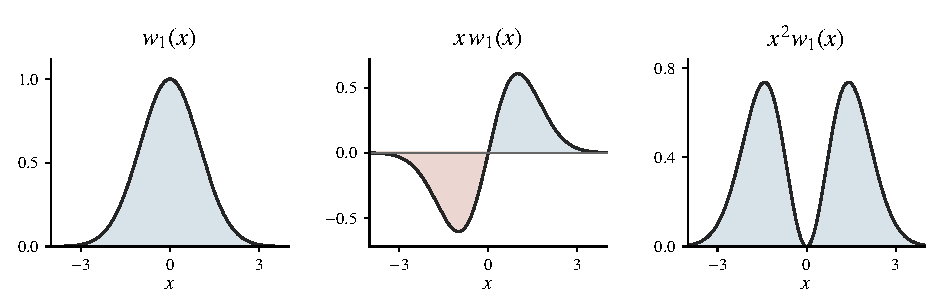
\includegraphics[width=\linewidth]{manuscript/figures/gaussian-weights.pdf}
\caption{The Gaussian weight at $h=1$ and its first two polynomial
integrands. The negative and positive contributions of $xw_1(x)$ cancel.
The integrand $x^2w_1(x)$ is positive away from zero.
Dividing their whole-line integrals by the same positive normalization
gives $\mathbb E_1(x)=0$ and $\mathbb E_1(x^2)=1$.}
\label{fig:gaussian-moment-integrands}
\end{figure}

The expression annihilated by elimination is
\[
 hg'-xg=hg'+I'g,
 \qquad I=-S=-x^2/2.
\]
It uses only multiplication and polynomial differentiation.
These operations define the corresponding relations over any field of
characteristic zero.

\subsection{The algebraic Gaussian complex}

Let $k$ be a field of characteristic zero. In this section,
$\hbar\in k$ is a fixed nonzero scalar of degree zero.
The polynomial algebra $k[x]$ has basis $1,x,x^2,\ldots$, with
$x^i x^j=x^{i+j}$ and $|x|=0$.

Adjoin a generator $\xi$ of degree $-1$, subject to $\xi^2=0$ and
$x\xi=\xi x$. The resulting graded algebra is
\[
 G=k[x]\otimes_k\Lambda(\xi)=k[x]\oplus\xi k[x].
\]
Here $\Lambda(\xi)=k\oplus k\xi$ is the exterior algebra.
The multiplication is
\[
 (f+\xi g)(u+\xi v)=fu+\xi(fv+gu).
\]
Thus $G^0=k[x]$, $G^{-1}=\xi k[x]$, and every other degree is zero.

Define the derivatives by
\[
 \begin{gathered}
 \partial_x(f+\xi g)=f'+\xi g',\qquad
 \partial_\xi(f+\xi g)=g,\\
 1'=0,\qquad (x^n)'=n x^{n-1}\quad(n\geq1).
 \end{gathered}
\]
They have degrees zero and one, respectively.
For homogeneous $a,b$, the odd derivative satisfies
\[
 \partial_\xi(ab)=(\partial_\xi a)b+(-1)^{|a|}a\partial_\xi b.
\]
Checking $a=f$ and $a=\xi g$ in the multiplication formula proves this
identity. The ordinary derivative satisfies the same rule without a sign.

Put $S=x^2/2$ and $I=-S$.
The stationary equation $S'(x)=0$ is $x=0$.
The degree-one derivation
$d_{\mathrm{cl}}=I'\partial_\xi=-x\partial_\xi$ records this equation
through $d_{\mathrm{cl}}\xi=-x$.
Its square is zero, and its cohomology is $k$ in degree zero.
Indeed, multiplication by $-x$ is injective on $k[x]$, and its cokernel
is $k[x]/(x)=k$.

For $k=\mathbb R$ and $\hbar=h>0$, the real Gaussian relation
annihilates $\hbar g'+I'g=\hbar g'-xg$ for every polynomial $g$.
Retain the same relation over $k$ by defining the Gaussian differential
\begin{equation}\label{eq:gaussian-differential}
 \delta=-x\partial_\xi+\hbar\partial_x\partial_\xi,
 \qquad \delta(f+\xi g)=\hbar g'-xg.
\end{equation}
Its output contains no $\xi$, so $\delta^2=0$.
The relation $\delta\xi=-x$ survives, but
\[
 \delta(x\xi)=\hbar-x^2,
 \qquad
 (\delta x)\xi+x\delta\xi=-x^2.
\]
The differential therefore fails the Leibniz rule by the nonzero scalar
$\hbar$.

An algebraic Gaussian functional supplies the quotient by these relations.
For a polynomial $f$, define
\begin{equation}\label{eq:gaussian-functional}
 \mathcal E_\hbar(f+\xi g)
 =\left.\left(\sum_{j\geq0}
       \frac{\hbar^j}{2^j j!}\partial_x^{2j}f\right)\right|_{x=0}.
\end{equation}
The sum is finite for each polynomial, and evaluation at $x=0$ extracts
its constant coefficient. This defines a $k$-linear map $G\to k$, where
$k$ is concentrated in degree zero with zero differential.

Direct differentiation gives
\[
 \mathcal E_\hbar(x^{2m})
 =\frac{(2m)!}{2^m m!}\hbar^m
 =(2m-1)!!\,\hbar^m,
 \qquad \mathcal E_\hbar(x^{2m+1})=0.
\]
The notation $(2m-1)!!$ means the product of the positive odd integers
at most $2m-1$, with $(-1)!!=1$.
In particular, $\mathcal E_\hbar(1)=1$.

These formulas imply
\begin{equation}\label{eq:gaussian-ward}
 \mathcal E_\hbar(xg)=\hbar\mathcal E_\hbar(g'),
 \qquad \mathcal E_\hbar\delta=0.
\end{equation}
For $g=x^n$, both sides vanish when $n$ is even.
When $n=2m+1$, the equality is
$(2m+1)!!\hbar^{m+1}=(2m+1)(2m-1)!!\hbar^{m+1}$.
Linearity proves the identity for every $g$.
Equation~\eqref{eq:gaussian-ward} is the Gaussian Ward identity in this
algebraic setting.

For $k=\mathbb R$ and $\hbar=h>0$, the algebraic functional agrees with
the normalized integral:
\[
 \mathcal E_h(f)=\mathbb E_h(f)
 \qquad(f\in\mathbb R[x]).
\]
Indeed, for a normalized linear functional $L$ satisfying the Gaussian
relation, put $m_n=L(x^n)$.
These values, called its moments, satisfy
\[
 m_0=1,\qquad m_1=0,\qquad
 m_{n+1}=hn\,m_{n-1}\quad(n\geq1).
\]
Both functionals satisfy these equations, which determine their values
on the monomial basis.
The algebraic definition remains valid for every characteristic-zero
field $k$ and every nonzero $\hbar\in k$.

\begin{proposition}\label{prop:gaussian-cohomology}
The functional $\mathcal E_\hbar$ induces an isomorphism
$H^0(G,\delta)\cong k$. All other cohomology groups vanish.
Polynomial multiplication does not induce multiplication on
$H^0(G,\delta)$.
\end{proposition}

\begin{proof}
For a nonzero polynomial $g$ of degree $d$, the highest term of
$\hbar g'-xg$ has degree $d+1$ and nonzero coefficient.
Thus $\delta:G^{-1}\to G^0$ is injective.

The boundary $\delta\xi=-x$ gives $[x]=0$.
For $n\geq1$,
\[
 \delta(\xi x^n)=\hbar n x^{n-1}-x^{n+1}
\]
so $[x^{n+1}]=\hbar n[x^{n-1}]$.
Every class is therefore a scalar multiple of $[1]$.
Since $\mathcal E_\hbar$ annihilates boundaries and sends $1$ to $1$,
the class $[1]$ is nonzero. This proves the cohomology statement.

If multiplication descended, $[x]=0$ would imply $[x^2]=0$.
The recurrence instead gives $[x^2]=\hbar[1]\ne0$.
Equivalently, the subspace $\operatorname{im}\delta\subset k[x]$
contains $x$ but does not contain $x^2$.
It is not an ideal.
\end{proof}

At $\hbar=0$, the same complex becomes the classical complex, and
its degree-zero quotient is an algebra.
For nonzero $\hbar$, the functional remains a normalized map of complexes,
but $\mathcal E_\hbar(x^2)\ne\mathcal E_\hbar(x)^2$.
The construction uses finite polynomial differentiation.
No integration measure is part of its definition.

In homological notation, $G_j=G^{-j}$ places $\xi$ in degree one
and $\delta$ in degree $-1$.
This regrading preserves parity and every displayed sign, and
identifies $H_0$ with $H^0$.

\section{The bracket of a second-order operator}
\label{sec:gaussian-bv-algebra}

The discrepancy in $\delta(x\xi)$ comes from
$\Delta=\partial_x\partial_\xi$.
To calculate this discrepancy on several variables, fix an integer
$n\geq1$ and let
\[
 A=k[x_1,\ldots,x_n]\otimes_k\Lambda(\xi_1,\ldots,\xi_n),
 \qquad |x_i|=0,\quad |\xi_i|=-1.
\]
The exterior relations are
$\xi_i\xi_j=-\xi_j\xi_i$ and $\xi_i^2=0$.
Each element is a unique sum of polynomials times ordered products
$\xi_{i_1}\cdots\xi_{i_r}$ with $i_1<\cdots<i_r$.
The product satisfies $ab=(-1)^{|a||b|}ba$ for homogeneous elements.
This identity defines graded commutativity.

The left odd derivative removes an occurrence with its position sign:
\[
 \partial_{\xi_i}(\xi_{j_1}\cdots\xi_{j_r})
 =\sum_{\ell=1}^r(-1)^{\ell-1}\delta_{i,j_\ell}
   \xi_{j_1}\cdots\widehat{\xi_{j_\ell}}\cdots\xi_{j_r}.
\]
Here $\delta_{i,j}$ equals one for $i=j$ and zero otherwise, and the hat
means omission. Extend the derivative $k[x_1,\ldots,x_n]$-linearly.
Splitting the removed positions between two factors proves its graded
Leibniz rule.

Removing two distinct positions in opposite orders changes
the sign, so
\[
 \partial_{\xi_i}^2=0,
 \qquad
 \partial_{\xi_i}\partial_{\xi_j}
 =-\partial_{\xi_j}\partial_{\xi_i}.
\]
The even derivatives $\partial_{x_i}$ commute with all these derivatives.
Consequently,
\[
 \Delta=\sum_{i=1}^n\partial_{x_i}\partial_{\xi_i},
 \qquad |\Delta|=1,
 \qquad \Delta1=0,
 \qquad \Delta^2=0.
\]
For the last equality, the terms with repeated index vanish and the
terms with distinct indices cancel in pairs.

Applying the two Leibniz rules gives
\[
 \begin{split}
 \Delta(ab)={}&(\Delta a)b+(-1)^{|a|}a\Delta b\\
 &+\sum_{i=1}^n\left(
    (\partial_{\xi_i}a)(\partial_{x_i}b)
    +(-1)^{|a|}(\partial_{x_i}a)(\partial_{\xi_i}b)\right).
 \end{split}
\]

Define the degree-one bracket by this failure of the Leibniz rule:
\begin{equation}\label{eq:gaussian-derived-bracket}
 \{a,b\}=(-1)^{|a|}
 \left(\Delta(ab)-(\Delta a)b-(-1)^{|a|}a\Delta b\right).
\end{equation}
The explicit formula is
\begin{equation}\label{eq:gaussian-coordinate-bracket}
 \{a,b\}=\sum_{i=1}^n\left(
  (\partial_{x_i}a)(\partial_{\xi_i}b)
  +(-1)^{|a|}(\partial_{\xi_i}a)(\partial_{x_i}b)\right).
\end{equation}
In particular, $\{x_i,\xi_j\}=\delta_{i,j}$ and
$\{\xi_j,x_i\}=-\delta_{i,j}$.

Moving homogeneous derivatives past each other in this formula gives
\begin{equation}\label{eq:gaussian-bracket-skew-leibniz}
 \begin{split}
 \{a,b\}&=-(-1)^{(|a|+1)(|b|+1)}\{b,a\},\\
 \{a,bc\}&=\{a,b\}c+(-1)^{(|a|+1)|b|}b\{a,c\}.
 \end{split}
\end{equation}
For example, the term $(\partial_{x_i}a)b\partial_{\xi_i}c$
acquires $(-1)^{|a||b|}$ when $b$ moves to its left.
Its Leibniz sign $(-1)^{|b|}$ gives the second sign in
\eqref{eq:gaussian-bracket-skew-leibniz}.
The term with $\partial_{\xi_i}a$ acquires
$(-1)^{(|a|+1)|b|}$ directly.
The first identity follows by the same reorderings applied to the two
terms of~\eqref{eq:gaussian-coordinate-bracket}.

Substituting the bracket definition into the second identity gives
\begin{equation}\label{eq:gaussian-seven-term}
 \begin{split}
 \Delta(abc)={}&\Delta(ab)c+(-1)^{|a|}a\Delta(bc)
       +(-1)^{(|a|+1)|b|}b\Delta(ac)\\
 &-(\Delta a)bc-(-1)^{|a|}a(\Delta b)c
       -(-1)^{|a|+|b|}ab\Delta c.
 \end{split}
\end{equation}
This is the seven-term identity.
It says that the failure of $\Delta$ to be a derivation is itself a
derivation in either input, with the stated graded signs.

\begin{definition}\label{def:gaussian-bv}
A cohomological Batalin--Vilkovisky algebra, abbreviated BV algebra,
is a unital graded commutative $k$-algebra $B$ with a degree-one
$k$-linear operator $\Delta$.
The operator satisfies
$\Delta1=0$, $\Delta^2=0$, and~\eqref{eq:gaussian-seven-term}.
Its BV bracket is~\eqref{eq:gaussian-derived-bracket}.
An operator satisfying the seven-term identity and annihilating the unit
is said here to have differential order at most two.
\end{definition}

The algebra $A$ above is a BV algebra.

\begin{proposition}\label{prop:gaussian-bv-identities}
In a BV algebra the bracket has the two properties in
\eqref{eq:gaussian-bracket-skew-leibniz} and satisfies
\begin{align}
 \Delta\{a,b\}
 &=\{\Delta a,b\}+(-1)^{|a|+1}\{a,\Delta b\},
 \label{eq:gaussian-delta-bracket}\\
 \{a,\{b,c\}\}
 &=\{\{a,b\},c\}
  +(-1)^{(|a|+1)(|b|+1)}\{b,\{a,c\}\}.
 \label{eq:gaussian-jacobi}
\end{align}
The last identity is the Jacobi identity for a bracket of degree one.
\end{proposition}

\begin{proof}
Graded commutativity in~\eqref{eq:gaussian-derived-bracket} gives the
first identity in~\eqref{eq:gaussian-bracket-skew-leibniz}.
Rearranging~\eqref{eq:gaussian-seven-term} gives the second.

For homogeneous operators $U,V,W$ of degrees $u,v,w$, define
$[U,V]=UV-(-1)^{|U||V|}VU$.
Expansion gives
\[
 [U,[V,W]]
 =UVW-(-1)^{vw}UWV-(-1)^{u(v+w)}VWU
       +(-1)^{u(v+w)+vw}WVU.
\]
Expanding $[[U,V],W]+(-1)^{uv}[V,[U,W]]$ gives these four terms:
the two copies of $VUW$ and the two copies of $WUV$ cancel.
Thus the graded commutator satisfies the Jacobi identity.

Let $m_a$ denote multiplication by $a$, and put $H_a(b)=\{a,b\}$.
The bracket Leibniz rule and its definition imply
\begin{equation}\label{eq:gaussian-multiplication-commutators}
 [H_a,m_b]=m_{\{a,b\}},
 \qquad [\Delta,m_a]=m_{\Delta a}+(-1)^{|a|}H_a.
\end{equation}
Direct expansion of the double commutator gives
$[\Delta,[\Delta,m_a]]=[\Delta^2,m_a]=0$.
Using~\eqref{eq:gaussian-multiplication-commutators} twice gives
\[
 0=(-1)^{|a|+1}H_{\Delta a}+(-1)^{|a|}[\Delta,H_a].
\]
Hence $[\Delta,H_a]=H_{\Delta a}$, which is
\eqref{eq:gaussian-delta-bracket} on an input $b$.

Write $p=|a|$ and $q=|b|$.
Substitute $H_b=(-1)^q([\Delta,m_b]-m_{\Delta b})$ and use
the commutator Jacobi identity. The result is
\[
 \begin{split}
 [H_a,H_b]={}&H_{\{a,b\}}
  +(-1)^{p+q}m_{\{\Delta a,b\}}\\
 &+(-1)^{p+q+1}m_{\Delta\{a,b\}}
  -(-1)^q m_{\{a,\Delta b\}}.
 \end{split}
\]
The three multiplication operators cancel by
\eqref{eq:gaussian-delta-bracket}.
Thus $[H_a,H_b]=H_{\{a,b\}}$.
Applying this equality to $c$ proves~\eqref{eq:gaussian-jacobi}.
\end{proof}

\section{Actions and the master equation}
\label{sec:gaussian-master-equation}

Let $(B,\Delta)$ be a BV algebra.
Suppose $Q:B\to B$ is a degree-one derivation satisfying
\[
 Q1=0,\qquad Q^2=0,\qquad Q\Delta+\Delta Q=0.
\]

From this section onward, $\hbar$ is a formal central variable of degree
zero, unless a specialization is stated.
Use degreewise completion, so $B[[\hbar]]^m=B^m[[\hbar]]$.
Its elements in degree $m$ are sequences
$\sum_{j\geq0}\hbar^j b_j$ with $b_j\in B^m$.
Multiplication and brackets use finite convolution sums at each power
of $\hbar$. The operators $Q$ and $\Delta$ extend coefficientwise.
An action is a series
$I=\sum_{j\geq0}\hbar^jI_j\in B^0[[\hbar]]$.

The compatibility of $Q$ with the bracket is
\begin{equation}\label{eq:gaussian-q-bracket}
 Q\{a,b\}=\{Qa,b\}+(-1)^{|a|+1}\{a,Qb\}.
\end{equation}
To prove it, the derivation rule gives $[Q,m_a]=m_{Qa}$.
The commutator Jacobi identity then gives
\[
 [Q,[\Delta,m_a]]=-[\Delta,m_{Qa}].
\]
Insert~\eqref{eq:gaussian-multiplication-commutators} on both sides.
The multiplication terms cancel because $Q\Delta a=-\Delta Qa$,
leaving $[Q,H_a]=H_{Qa}$.
This is~\eqref{eq:gaussian-q-bracket}.

For a degree-zero action $I$, define its curvature and observable operator by
\begin{equation}\label{eq:gaussian-curvature}
 \mathcal F(I)=QI+\frac12\{I,I\}+\hbar\Delta I,
 \qquad d_I=Q+\{I,-\}+\hbar\Delta.
\end{equation}
The equation $\mathcal F(I)=0$ is the quantum master equation.
For an action $I_0\in B^0$, the equation
$QI_0+\tfrac12\{I_0,I_0\}=0$ is the classical master equation.
All terms in either equation have degree one.

\begin{proposition}\label{prop:gaussian-master-square}
For every degree-zero action,
\begin{equation}\label{eq:gaussian-master-square}
 d_I^2=\{\mathcal F(I),-\}.
\end{equation}
An action satisfying the quantum master equation therefore defines a
complex $(B[[\hbar]],d_I)$.
\end{proposition}

\begin{proof}
Put $D=Q+\hbar\Delta$. Its square is
$Q^2+\hbar(Q\Delta+\Delta Q)+\hbar^2\Delta^2=0$.
Both $D$ and $H_I$ have degree one. Their remaining contributions are
\[
 \begin{split}
 d_I^2
 &=D^2+[Q,H_I]+\hbar[\Delta,H_I]+\tfrac12[H_I,H_I]\\
 &=H_{QI}+\hbar H_{\Delta I}+\tfrac12H_{\{I,I\}}
 =H_{\mathcal F(I)}.
 \end{split}
\]
\end{proof}

The converse of this proposition requires an additional condition:
$d_I^2=0$ says that $\mathcal F(I)$ brackets to zero with every element.
Such an element is called bracket-central.
It need not be zero.

On $G[[\hbar]]$, take $Q=0$ and $I=-x^2/2$.
Then $\{I,-\}=-x\partial_\xi$ and $\Delta I=\{I,I\}=0$, so
\[
 d_I=-x\partial_\xi+\hbar\partial_x\partial_\xi.
\]
This operator preserves the polynomial subcomplex $G[\hbar]$.
For $\alpha\in k^\times$, evaluation $\hbar\mapsto\alpha$ gives a
map from this subcomplex to $G$ with differential
$-x\partial_\xi+\alpha\partial_x\partial_\xi$.
It recovers~\eqref{eq:gaussian-differential} with scalar parameter $\alpha$.
No evaluation of arbitrary elements of $G[[\hbar]]$ is used.

The multiplication defect of any $d_I$ is explicit:
\begin{equation}\label{eq:gaussian-observable-product}
 d_I(ab)-(d_Ia)b-(-1)^{|a|}a\,d_Ib
 =(-1)^{|a|}\hbar\{a,b\}.
\end{equation}
The terms $Q$ and $H_I$ are derivations, leaving only the defect of
$\hbar\Delta$.
If homogeneous $a,b$ are cycles, then $ab$ is a cycle exactly when
$\{a,b\}=0$.
Indeed, multiplication by $\hbar$ is injective on $B[[\hbar]]$, since
it shifts every coefficient by one place.
Even when the product is a cycle, the Gaussian example shows that its
class can depend on the representatives.

\section{A finite heat homotopy and its residual variables}
\label{sec:gaussian-heat}

The elimination of an acyclic pair can be expressed as a homotopy with
an explicit scale parameter.
Use the real field in this section and the cochain space
\[
 E^0=\mathbb R u\oplus\mathbb R r,
 \qquad E^1=\mathbb R v\oplus\mathbb R s.
\]
Give the displayed basis the Euclidean inner product.
For a fixed real number $a>0$, define
\[
 Qu=av,\quad Qv=Qr=Qs=0,
 \qquad qv=au,\quad qu=qr=qs=0.
\]

The map $Q$ has degree one, and its adjoint $q$ has degree $-1$.
These formulas give $Q^2=q^2=0$.
The operator $H=Qq+qQ$ acts by $\lambda=a^2$ on
$\mathbb R u\oplus\mathbb R v$, and by zero on
$\mathbb R r\oplus\mathbb R s$.

For real $t\geq0$, put $\kappa_t=e^{-\lambda t}$ and define
$K_t^{\mathrm{op}}=e^{-tH}$ by this diagonal action.
The exponential estimate~\eqref{eq:gaussian-exponential-remainder} gives
\[
 |\kappa_{t+u}-\kappa_t+\lambda\kappa_tu|
 \leq2\lambda^2u^2
 \qquad\left(t,t+u\geq0,\quad |u|\leq\frac1{2\lambda}\right).
\]
Dividing by $|u|$ proves that the difference quotient tends to
$-\lambda\kappa_t$ as $u\to0$.
This limit defines $\partial_t\kappa_t$, with a right derivative at zero.
Consequently,
\[
 \partial_tK_t^{\mathrm{op}}=-HK_t^{\mathrm{op}},
 \qquad K_0^{\mathrm{op}}=1.
\]
This evolution equation is the heat equation for the operator $H$.

The first exponential estimate also gives
$|\kappa_t-\kappa_s|\leq\lambda|t-s|$ for $s,t\geq0$.
Thus $\kappa_t$ has the tagged integral constructed above.
Sum the difference-quotient remainder over a partition of
$[\epsilon,L]$, with $0\leq\epsilon<L<\infty$.
The increments telescope, and the total error is at most
$2\lambda^2(L-\epsilon)|P|$.
Taking the limit as the mesh tends to zero proves
\[
 \int_\epsilon^L\kappa_t\,dt
 =\frac{\kappa_\epsilon-\kappa_L}{\lambda}.
\]

Set
\[
 \rho_{\epsilon,L}
 =\frac{\kappa_\epsilon-\kappa_L}{\lambda},
 \qquad
 P_{\epsilon,L}^{\mathrm{op}}
 =\int_\epsilon^L q e^{-tH}\,dt
 =\rho_{\epsilon,L}q.
\]
The integral is taken entrywise in the displayed basis.
The sole nonzero entry of $qe^{-tH}$ sends $v$ to $a\kappa_tu$.

Directly on $u,v,r,s$,
\begin{equation}\label{eq:gaussian-heat-homotopy}
 QP_{\epsilon,L}^{\mathrm{op}}+P_{\epsilon,L}^{\mathrm{op}}Q
 =K_\epsilon^{\mathrm{op}}-K_L^{\mathrm{op}}.
\end{equation}
Both sides multiply $u,v$ by
$\lambda\rho_{\epsilon,L}=\kappa_\epsilon-\kappa_L$ and annihilate $r,s$.

The insertion of $q$ supplies the degree $-1$ required by a homotopy.
In contrast, $\int_\epsilon^L e^{-tH}\,dt$ has degree zero and
commutes with $Q$, so its graded commutator with $Q$ is zero.

Let $\pi_E$ be the projection onto $\mathbb R r\oplus\mathbb R s$.
The inequality $e^{\lambda L}\geq1+\lambda L$ gives
$\kappa_L\to0$ as $L\to\infty$.
Consequently,
\[
 K_L^{\mathrm{op}}\longrightarrow\pi_E,
 \qquad
 P_{0,\infty}^{\mathrm{op}}v=a^{-1}u,
 \qquad
 QP_{0,\infty}^{\mathrm{op}}+P_{0,\infty}^{\mathrm{op}}Q=1-\pi_E.
\]
The classes of $r$ and $s$ span $H^0(E,Q)$ and $H^1(E,Q)$,
respectively. They are the residual variables.

To turn the heat operators into contractions on polynomial functions,
specify their kernel tensors using a degree-$-1$ bilinear pairing
$\omega:E\otimes E\to\mathbb R$:
\[
 \omega(u,v)=\omega(r,s)=1,
 \qquad \omega(v,u)=\omega(s,r)=-1,
\]
with every other basis pairing zero.
For a tensor $M=\sum_i A_i\otimes B_i$ and a homogeneous vector $e$,
use the convention
\[
 M\star e=(-1)^{|e|}\sum_i A_i\omega(B_i,e).
\]

The kernel tensors for the two operators are
\[
 \begin{split}
 K_t&=-\kappa_t(u\otimes v+v\otimes u)
             -(r\otimes s+s\otimes r),\\
 P_{\epsilon,L}&=\int_\epsilon^L(q\otimes1)K_t\,dt
             =-a\rho_{\epsilon,L}u\otimes u.
 \end{split}
\]
Their degrees are one and zero, respectively.
The rule $\star$ gives operators of degrees zero and $-1$, as required.
For instance, $K_t\star u=\kappa_tu$,
$K_t\star v=\kappa_tv$, and
$P_{\epsilon,L}\star v=a\rho_{\epsilon,L}u$.

The tensor differential is
\[
 Q_{\otimes}(e\otimes f)=Qe\otimes f+(-1)^{|e|}e\otimes Qf.
\]
It therefore satisfies
\[
 Q_{\otimes}P_{\epsilon,L}
 =-a^2\rho_{\epsilon,L}(v\otimes u+u\otimes v)
 =K_\epsilon-K_L.
\]

The graded dual has
$(E^\vee)^j=\operatorname{Hom}_{\mathbb R}(E^{-j},\mathbb R)$.
Let $x,z,\xi,\eta$ be dual to $u,r,v,s$, respectively.
Thus the polynomial functions form
\[
 A=\mathbb R[x,z]\otimes\Lambda(\xi,\eta),
 \qquad |x|=|z|=0,\quad |\xi|=|\eta|=-1.
\]
The dual differential is
$(Q_A\phi)(e)=-(-1)^{|\phi|}\phi(Qe)$ on linear functions,
extended as a derivation. It gives $Q_A\xi=ax$, with the other
three generators closed, so $Q_A=ax\partial_\xi$.

Write $\partial_u=\partial_x$, $\partial_r=\partial_z$,
$\partial_v=\partial_\xi$, and $\partial_s=\partial_\eta$.
For $M=\sum_i A_i\otimes B_i$, define its contraction operator by
$\partial_M=\tfrac12\sum_i\partial_{A_i}\partial_{B_i}$.
The normalization used for the odd kernel is $\Delta_t=-\partial_{K_t}$.
For the even propagator it is $B_{\epsilon,L}=\partial_{P_{\epsilon,L}}$.

These definitions give
\begin{equation}\label{eq:gaussian-scale-operators}
 \Delta_t=\kappa_t\partial_x\partial_\xi+
                    \partial_z\partial_\eta,
 \qquad
 B_{\epsilon,L}=-\frac{a\rho_{\epsilon,L}}2\partial_x^2.
\end{equation}
Both $Q_A$ and $\Delta_t$ have degree one, while $B_{\epsilon,L}$
has degree zero.

Their direct commutators are
\begin{equation}\label{eq:gaussian-scale-commutators}
 \begin{gathered}
 Q_A^2=\Delta_t^2=Q_A\Delta_t+\Delta_tQ_A=0,\\
 [Q_A,B_{\epsilon,L}]=\Delta_\epsilon-\Delta_L,
 \qquad [B_{\epsilon,L},\Delta_t]=0.
 \end{gathered}
\end{equation}
For the nonconstant coefficient in $Q_A$, the commutator calculation is
\[
 [\partial_x^2,x\partial_\xi]=2\partial_x\partial_\xi.
\]
It gives
$[Q_A,B_{\epsilon,L}]=a^2\rho_{\epsilon,L}\partial_x\partial_\xi$.
The other identities follow from commutation of even derivatives and
anticommutation of odd derivatives.

\begin{proposition}\label{prop:gaussian-intertwining}
On $A[\hbar]$, on $A[\hbar,\hbar^{-1}]$, and coefficientwise on
$A[[\hbar]]$, the operator
$T_{\epsilon,L}=\exp(\hbar B_{\epsilon,L})$ satisfies
\begin{equation}\label{eq:gaussian-intertwining}
 (Q_A+\hbar\Delta_L)T_{\epsilon,L}
 =T_{\epsilon,L}(Q_A+\hbar\Delta_\epsilon).
\end{equation}
It is an invertible linear map with inverse
$\exp(-\hbar B_{\epsilon,L})$, and it preserves the unit.
\end{proposition}

\begin{proof}
Each $B_{\epsilon,L}$ lowers the polynomial degree in $x$ by two.
Its exponential therefore has finitely many nonzero terms on every
polynomial. On a formal series in $\hbar$, the coefficient of
$\hbar^N$ uses only the terms indexed by $0\leq j\leq N$.
The two exponential series multiply to one by the binomial identity,
and both fix $1$.

Abbreviate $B=B_{\epsilon,L}$ and $C=[Q_A,B]$.
Equation~\eqref{eq:gaussian-scale-commutators} gives $[B,C]=0$.
Expanding the commutator with a power gives
$[Q_A,B^j]=jB^{j-1}C$.
Hence $Q_AT=TQ_A+\hbar TC$.
Since $\Delta_L$ commutes with $T$, this yields
\[
 (Q_A+\hbar\Delta_L)T
 =T\bigl(Q_A+\hbar(C+\Delta_L)\bigr)
 =T(Q_A+\hbar\Delta_\epsilon).
\]
\end{proof}

Put $A_{\mathrm{res}}=\mathbb R[z]\otimes\Lambda(\eta)$ and
$\Delta_{\mathrm{res}}=\partial_z\partial_\eta$.
The following elimination maps act on each pair of source and target:
\[
 \begin{gathered}
 (A[\hbar],A_{\mathrm{res}}[\hbar]),\\
 (A[\hbar,\hbar^{-1}],A_{\mathrm{res}}[\hbar,\hbar^{-1}]),\\
 (A[[\hbar]],A_{\mathrm{res}}[[\hbar]]).
 \end{gathered}
\]
The third pair uses degreewise series whose coefficients are polynomials.
Every output coefficient of a contraction exponential is a finite sum.
Let $\pi_A$ evaluate $x=\xi=0$ on each polynomial or series coefficient.

At infinite scale, $\pi_A$ intertwines
$d_\infty=ax\partial_\xi+\hbar\Delta_{\mathrm{res}}$ with
$\hbar\Delta_{\mathrm{res}}$.
At a finite scale $t$, the corresponding map is
\begin{equation}\label{eq:gaussian-residual-map}
 \mathcal P_t
 =\pi_A\exp\left(-\frac{\hbar\kappa_t}{2a}\partial_x^2\right).
\end{equation}
Taking $L\to\infty$ in the finite polynomial identities proves
\[
 \hbar\Delta_{\mathrm{res}}\mathcal P_t
 =\mathcal P_t(Q_A+\hbar\Delta_t).
\]
Plain evaluation fails at finite scale: applying it to
$(Q_A+\hbar\Delta_t)(x\xi)$ gives $\hbar\kappa_t$.

The algebraic covariance of $\mathcal P_t$ is negative:
\[
 \mathcal P_t(x)=0,\qquad
 \mathcal P_t(x^2)=-\frac{\hbar\kappa_t}{a}.
\]
The positive coefficient in $Q_A=ax\partial_\xi$ forces this sign
through~\eqref{eq:gaussian-scale-commutators}.
The opening Gaussian functional instead has covariance $+\hbar$.
For positive real $\hbar$ and $a$, $\mathcal P_t$ sends the nonnegative
polynomial $x^2$ to a negative number.
It cannot therefore be the normalized integral of a nonnegative weight.

The residual map is a cohomology isomorphism, with a direct homotopy.
First let $i_A:A_{\mathrm{res}}\to A$ be inclusion.
Write an element of $A$ uniquely as $f+\xi g$, with
$f,g\in A_{\mathrm{res}}[x]$ and $\xi$ placed on the left.
Define a degree-$-1$ map
\[
 h_0(f+\xi g)=\frac{\xi}{a}\frac{f-f|_{x=0}}{x}.
\]
The quotient is a polynomial because its numerator has zero constant
coefficient in $x$.

Extend $i_A$ and $h_0$ coefficientwise to each of the three coefficient
extensions. The formulas below therefore hold on each source and target pair.

For $d_K=ax\partial_\xi$, direct substitution gives
$d_Kh_0+h_0d_K=1-i_A\pi_A$.
The residual odd operator satisfies
$\Delta_{\mathrm{res}}(\xi g)=-\xi\Delta_{\mathrm{res}}g$,
so $\Delta_{\mathrm{res}}h_0+h_0\Delta_{\mathrm{res}}=0$.
Thus $d_\infty h_0+h_0d_\infty=1-i_A\pi_A$.

Conjugating this identity by
$T_{t,\infty}=\exp(-\hbar\kappa_t\partial_x^2/(2a))$ gives
\[
 (Q_A+\hbar\Delta_t)h_t+h_t(Q_A+\hbar\Delta_t)
 =1-i_A\mathcal P_t,
 \qquad h_t=T_{t,\infty}^{-1}h_0T_{t,\infty}.
\]
Here $T_{t,\infty}^{-1}i_A=i_A$, and $\mathcal P_ti_A=1$.
These equations prove the cohomology isomorphism.

\section{The effective interaction and the linear observable map}
\label{sec:gaussian-effective}

For a real polynomial $I$, change the quadratic action $S$ to $S-I$.
At a fixed positive real number $h$, the numerical exponential satisfies
\[
 e^{-(S-I)/h}=e^{-S/h}e^{I/h}.
\]
Thus adding real interactions multiplies their numerical weights.
The algebraic elimination problem uses formal exponential weights and
the linear contraction $T=T_{\epsilon,L}$.
It asks for a degree-zero effective interaction $W(I)$ satisfying
\[
 e^{W(I)/\hbar}=T(e^{I/\hbar}).
\]
Recovering $W(I)$ therefore requires a logarithm.

The coefficient algebra must admit arbitrarily high interaction powers
and negative powers of $\hbar$.
For the polynomial algebra $A$ above, these operations are defined
in
\[
 \mathcal A=A[\hbar,\hbar^{-1}][[t]].
\]
Here $t$ is an independent formal variable of degree zero.
At each power of $t$, the coefficient is a polynomial in the fields
and a finite Laurent polynomial in $\hbar$.
The lower bound on the powers of $\hbar$ may depend on the power of $t$.

Multiplication has a finite sum of coefficient products at each $t$-degree.
The $t$-adic topology means that coefficients below any fixed power of
$t$ eventually agree.
An interaction is an element $I\in t\mathcal A^0$.
Its exponential $e^{I/\hbar}$ is defined because its term of order $m$
has $t$-degree at least $m$.

The contraction $T$ acts coefficientwise on $\mathcal A$.
It is defined because every coefficient is polynomial in the fields.
Set
\begin{equation}\label{eq:gaussian-effective-action}
 Z_I=T(e^{I/\hbar}),\qquad
 W(I)=\hbar\log Z_I,
 \qquad
 \log(1+u)=\sum_{m\geq1}\frac{(-1)^{m+1}}{m}u^m.
\end{equation}
Since $T1=1$, one has $Z_I\in1+t\mathcal A^0$.
The logarithm and the inverse of $Z_I$ are therefore defined in the
$t$-adic topology. In particular, $W(I)\in t\mathcal A^0$.

Write the one-variable formal series as
\[
 E(s)=\sum_{m\geq0}\frac{s^m}{m!},\qquad
 L(s)=\sum_{m\geq1}\frac{(-1)^{m+1}}m s^m.
\]
Coefficientwise differentiation gives $E'=E$ and $L'=(1+s)^{-1}$.
The formal chain rule follows from the rule for powers: each coefficient
of a composition with zero constant term uses finitely many powers.
The product and chain rules therefore give
\[
 \frac{d}{ds}L(E(s)-1)=1,\qquad
 \frac{d}{ds}\left(E(L(s))(1+s)^{-1}\right)=0.
\]
For the inverse factor, differentiation of
$(1+s)(1+s)^{-1}=1$ gives derivative $-(1+s)^{-2}$.

The series $L(E(s)-1)$ and $E(L(s))(1+s)^{-1}$ have constant terms
zero and one, respectively. In characteristic zero, a series with derivative zero
has only its constant coefficient.
Hence $L(E(s)-1)=s$ and $E(L(s))=1+s$.
Substitution into $t\mathcal A^0$ preserves every coefficient identity.
Thus $W(I)$ is the unique element of $t\mathcal A^0$ with exponential
weight $Z_I$.

For $I=tJ$ with $J\in A[\hbar,\hbar^{-1}]^0$ independent of $t$,
linearity of $T$ gives
\[
 Z_{tJ}=1+\frac{t}{\hbar}T(J)
          +\frac{t^2}{2\hbar^2}T(J^2)+O(t^3).
\]
Here $O(t^3)$ denotes an element of the ideal $t^3\mathcal A$.
Inserting this expression into $\log(1+u)=u-u^2/2+O(u^3)$ yields
\begin{equation}\label{eq:gaussian-second-connected}
 W(tJ)=tT(J)+\frac{t^2}{2\hbar}
                   \bigl(T(J^2)-T(J)^2\bigr)+O(t^3).
\end{equation}
The second coefficient records the failure of $T$ to preserve the
product $J^2$.

The higher coefficients have the same partition structure.
Put $Z_n=\hbar^{-n}T(J^n)$ and $Z_0=1$.
For $n\geq1$, let $\Pi_n$ be the finite set of partitions of
$\{1,\ldots,n\}$ into nonempty blocks. Then
\begin{equation}\label{eq:gaussian-connected-coefficients}
 [t^n]\log Z_{tJ}
 =\frac1{n!}\sum_{\pi\in\Pi_n}
       (-1)^{|\pi|-1}(|\pi|-1)!
       \prod_{B\in\pi}Z_{|B|}.
\end{equation}

To derive this formula, expand the logarithm as a sum of powers of
$Z_{tJ}-1$. At power $r$, the coefficient distributes $n$ labeled
inputs among $r$ nonempty ordered blocks.
Each unordered partition has $r!$ orders, and the logarithm contributes
$(-1)^{r+1}/r$. Their product is
$(-1)^{r-1}(r-1)!$.
This proves~\eqref{eq:gaussian-connected-coefficients}.

The contraction itself gives a second description of these coefficients.
Put $b=-\hbar a\rho_{\epsilon,L}$, so $T=\exp(b\partial_x^2/2)$.
Since $J$ has degree zero, it belongs to $\mathcal C[x]$, where
$\mathcal C=\mathbb R[z,\hbar,\hbar^{-1}]$.
For $n\geq1$, distinguish the $n$ factors of $J^n$ using variables
$X_1,\ldots,X_n$ of degree zero.
Let $J_i$ be $J$ with $x$ replaced by $X_i$, leaving all other
coefficients fixed.
Let
\[
 \operatorname{ev}:\mathcal C[X_1,\ldots,X_n]\longrightarrow\mathcal C[x]
\]
be the $\mathcal C$-algebra map substituting $X_1=\cdots=X_n=x$.

For $F\in\mathcal C[X_1,\ldots,X_n]$, the monomial derivative rule gives
\[
 \partial_x\operatorname{ev}(F)
 =\operatorname{ev}\left(\sum_{i=1}^n\partial_{X_i}F\right).
\]
For a monomial $\prod_iX_i^{r_i}$, both sides are
$(\sum_i r_i)x^{\sum_i r_i-1}$ when $\sum_i r_i>0$.
Both are zero when every exponent is zero.
Iteration and linearity therefore give
\begin{equation}\label{eq:gaussian-labeled-contraction}
 Z_n=\hbar^{-n}\operatorname{ev}\left[
  \exp\left(\frac b2\left(\sum_{i=1}^n\partial_{X_i}\right)^2\right)
  \prod_{i=1}^nJ_i\right].
\end{equation}

Each summand of the operator in the exponential lowers total polynomial
degree by two. Its exponential is therefore finite on any input.
The operators $\partial_{X_i}$ commute, and
\[
 \frac b2\left(\sum_i\partial_{X_i}\right)^2
 =\sum_i\frac b2\partial_{X_i}^2
    +\sum_{i<j}b\partial_{X_i}\partial_{X_j}.
\]
For commuting operators $U,V$ that lower polynomial degree,
the binomial identity gives
\[
 \sum_{r\geq0}\frac{(U+V)^r}{r!}
 =\sum_{p,q\geq0}\frac{U^pV^q}{p!q!}
 =e^Ue^V
\]
on each polynomial. Every sum in this equality is finite on that input.
Repeated application proves the factorization
\begin{equation}\label{eq:gaussian-edge-factorization}
 \exp\left(\frac b2\left(\sum_i\partial_{X_i}\right)^2\right)
 =\prod_i\exp\left(\frac b2\partial_{X_i}^2\right)
    \prod_{i<j}\exp\left(b\partial_{X_i}\partial_{X_j}\right).
\end{equation}

A finite graph on labeled vertices $1,\ldots,n$ is specified here by
nonnegative integers $m_{ij}$ for $1\leq i\leq j\leq n$.
For $i<j$, there are $m_{ij}$ edges between $i$ and $j$.
The $m_{ii}$ edges from $i$ to itself are loops.
Thus the definition allows multiple edges and loops.
Its number of edges, number of loops, and degrees of vertices are
\[
 e=\sum_{i\leq j}m_{ij},\qquad
 \ell=\sum_i m_{ii},\qquad
 d_i=2m_{ii}+\sum_{j<i}m_{ji}+\sum_{j>i}m_{ij}.
\]
Each loop contributes twice to the degree of its vertex.

The selected loop and edge terms in~\eqref{eq:gaussian-edge-factorization} are
\[
 \frac{(b/2)^{m_{ii}}}{m_{ii}!}\partial_{X_i}^{2m_{ii}}
 \quad\text{and}\quad
 \frac{b^{m_{ij}}}{m_{ij}!}\partial_{X_i}^{m_{ij}}\partial_{X_j}^{m_{ij}}
 \quad(i<j).
\]
Multiplication of these explicit terms, followed by evaluation, assigns
the graph the weight
\begin{equation}\label{eq:gaussian-graph-weight}
 w(m)=\frac{\hbar^{-n}b^e}
             {2^\ell\prod_{i\leq j}m_{ij}!}
           \prod_{i=1}^n\partial_x^{d_i}J.
\end{equation}
Thus $Z_n$ is the sum of these weights.

For $J\ne0$ of $x$-degree $d$, a nonzero weight requires every $d_i\leq d$.
It follows that $2e=\sum_i d_i\leq nd$, so only finitely many graphs
contribute. If $J=0$, all weights vanish.

Vertices $i,j$ belong to the same connected component if there is a
sequence $i=i_0,\ldots,i_r=j$ such that
$m_{\min(i_{q-1},i_q),\max(i_{q-1},i_q)}>0$ for $1\leq q\leq r$.
The sequence with $r=0$ joins a vertex to itself.
It is an equivalence relation: reversing sequences proves symmetry,
and concatenating them proves transitivity.
Its equivalence classes partition the vertices.
A graph is connected when this partition has one block.
In particular, every one-vertex graph is connected, with any number of loops.

No edge joins two distinct components.
In~\eqref{eq:gaussian-graph-weight}, $n,e,\ell$ are therefore the sums
of their values on the components.
The factorial product and derivative product also separate by component.
Consequently the weight of a graph is the product of its component weights.
Define $C_n$ to be the sum of weights of connected graphs on $n$ labeled
vertices, for $n\geq1$.
Relabeling a vertex set by $1,\ldots,n$ preserves the weight because
each vertex carries the same polynomial $J$.

Conversely, a partition $\pi\in\Pi_n$ and a connected graph on each
block determine one graph on $\{1,\ldots,n\}$.
These two constructions are inverse. Weight factorization then gives
\begin{equation}\label{eq:gaussian-component-partition}
 Z_n=\sum_{\pi\in\Pi_n}\prod_{B\in\pi}C_{|B|}.
\end{equation}
The empty graph has weight $Z_0=1$.

To compute the generating series of this partition sum, expand
\[
 \exp\left(\sum_{j\geq1}\frac{C_j}{j!}t^j\right)
 =\sum_{r\geq0}\frac1{r!}
       \left(\sum_{j\geq1}\frac{C_j}{j!}t^j\right)^r.
\]
For $n\geq1$, a term in its coefficient of $t^n$ chooses positive
integers $n_1,\ldots,n_r$ with sum $n$.
There are $n!/(n_1!\cdots n_r!)$ ordered disjoint blocks of these sizes
covering $n$ labeled vertices.
This count follows by successively choosing the elements of each block.
Every partition into $r$ blocks has $r!$ orders, including when block
sizes coincide, because its blocks are distinct subsets.

The factor $1/r!$ removes those orders, while the factors $1/n_i!$
give the displayed count after division by $n!$.
Thus the coefficient of $t^n$ is
$\frac1{n!}\sum_{\pi\in\Pi_n}\prod_{B\in\pi}C_{|B|}$.
Each coefficient is finite, since $r\leq n$ and all $n_i\geq1$.
Equation~\eqref{eq:gaussian-component-partition} proves
\[
 Z_{tJ}=\exp\left(\sum_{n\geq1}\frac{C_n}{n!}t^n\right),
 \qquad [t^n]\log Z_{tJ}=\frac{C_n}{n!}\quad(n\geq1).
\]
This identifies~\eqref{eq:gaussian-connected-coefficients} with connected
graph sums.

Take $J=x^2$ to compute every graph on two vertices with nonzero weight.
A single vertex can carry zero loops or one loop.
Their weights are $x^2/\hbar$ and $b/\hbar$, since
$(b/(2\hbar))\partial_x^2(x^2)=b/\hbar$.
Hence $C_1=(x^2+b)/\hbar$.

On two vertices, a connected graph needs at least one edge between them.
The degree bound $d_i\leq2$ leaves just two possibilities:
\[
 \begin{array}{c|c|c}
 m_{12}&(m_{11},m_{22})&w(m)\\ \hline
 1&(0,0)&4b x^2/\hbar^2\\
 2&(0,0)&2b^2/\hbar^2
 \end{array}
\]
The first weight is $\hbar^{-2}b(2x)^2$.
The second is $\hbar^{-2}(b^2/2!)(2)^2$.

All other nonzero two-vertex graphs have no cross-edge and split into
two one-vertex components. Their total weight is $C_1^2$.
Therefore
\[
 C_2=\frac{4b x^2+2b^2}{\hbar^2},\qquad
 Z_2=C_1^2+C_2=\frac{x^4+6b x^2+3b^2}{\hbar^2}.
\]
Directly, $T(x^4)=x^4+(b/2)12x^2+(b^2/8)24$ gives the same result.
Writing $\beta=a\rho_{\epsilon,L}$, so $b=-\hbar\beta$, gives
\[
 [t^2]W(tx^2)=\frac{\hbar C_2}{2}
             =-2\beta x^2+\hbar\beta^2.
\]
Subtracting $T(J)^2$ in~\eqref{eq:gaussian-second-connected} has removed
exactly the graphs with two connected components.

The bracket at a real scale $\sigma\geq0$ means the bracket obtained from
$\Delta_\sigma$ by
\eqref{eq:gaussian-derived-bracket}. Scale labels on brackets indicate
this choice of operator.
Put $D_\sigma=Q_A+\hbar\Delta_\sigma$.

\begin{proposition}\label{prop:gaussian-qme-transport}
If $I\in t\mathcal A^0$ satisfies
\[
 Q_AI+\tfrac12\{I,I\}_\epsilon+\hbar\Delta_\epsilon I=0,
\]
then $W(I)$ satisfies the corresponding equation at scale $L$.
\end{proposition}

\begin{proof}
For any degree-zero element $I$ and integer $m\geq2$, induction using
the bracket Leibniz rule gives
\[
 \begin{split}
 Q_A(I^m)&=m I^{m-1}Q_AI,\\
 \Delta_\sigma(I^m)&=m I^{m-1}\Delta_\sigma I
              +\frac{m(m-1)}2 I^{m-2}\{I,I\}_\sigma.
 \end{split}
\]
For the second induction, apply the product formula to $I^m I$.
The new bracket term is
$\{I^m,I\}_\sigma=m I^{m-1}\{I,I\}_\sigma$.
It changes $m(m-1)/2$ to $m(m+1)/2$.
The cases $m=0,1$ use $Q_A1=\Delta_\sigma1=0$ and the definitions
of $Q_AI$ and $\Delta_\sigma I$ directly.

Summing the two identities in the exponential yields
\begin{equation}\label{eq:gaussian-exponential-qme}
 D_\sigma e^{I/\hbar}
 =\hbar^{-1}\left(Q_AI+\tfrac12\{I,I\}_\sigma+
                          \hbar\Delta_\sigma I\right)e^{I/\hbar}.
\end{equation}
Thus the assumed equation says $D_\epsilon e^{I/\hbar}=0$.
Equation~\eqref{eq:gaussian-intertwining} gives
$D_L e^{W(I)/\hbar}=D_LT e^{I/\hbar}=0$.
Apply~\eqref{eq:gaussian-exponential-qme} to $W(I)$ and multiply
by the invertible element $\hbar e^{-W(I)/\hbar}$.
\end{proof}

In the particular algebra $A$, every degree-zero interaction contains
only $x,z$. Its master equation is therefore automatic.

The transport proof depends only on specified BV operators and a unital
linear intertwiner. More generally, let $A'$ be a unital graded
commutative algebra over a field $k$ of characteristic zero.
Give it degree-one BV operators $\Delta'_\epsilon,\Delta'_L$ and a
degree-one derivation $Q'$ satisfying
\[
 (Q')^2=0,\qquad
 Q'\Delta'_\sigma+\Delta'_\sigma Q'=0
       \quad(\sigma=\epsilon,L).
\]
Each BV operator satisfies the unit, square-zero, and seven-term
conditions of Definition~\ref{def:gaussian-bv}.
Its derived bracket is denoted $\{-,-\}'_\sigma$.
Extend $Q'$ and both BV operators linearly over $k[\hbar,\hbar^{-1}]$,
with $|\hbar|=0$.

Suppose a degree-zero $k[\hbar,\hbar^{-1}]$-linear map
\[
 T':A'[\hbar,\hbar^{-1}]\longrightarrow A'[\hbar,\hbar^{-1}]
\]
satisfies
\[
 T'1=1,\qquad
 (Q'+\hbar\Delta'_L)T'=T'(Q'+\hbar\Delta'_\epsilon).
\]
For a formal variable $t$ of degree zero, set
$\mathcal A'^j=A'^j[\hbar,\hbar^{-1}][[t]]$ for each integer $j$.
Extend $Q',\Delta'_\epsilon,\Delta'_L,T'$ coefficientwise in $t$,
and use coefficient convolution for products and brackets.
These maps are continuous in the $t$-adic topology, since they preserve
every ideal $(t^N)$.

For $I'\in t\mathcal A'^0$, the exponential and logarithm exist because
only finitely many powers contribute to any coefficient of $t$.
Define $W'=\hbar\log T'(e^{I'/\hbar})$.
If
\[
 Q'I'+\tfrac12\{I',I'\}'_\epsilon+\hbar\Delta'_\epsilon I'=0,
\]
then the power calculation gives
$(Q'+\hbar\Delta'_\epsilon)e^{I'/\hbar}=0$.
Intertwining gives $(Q'+\hbar\Delta'_L)e^{W'/\hbar}=0$.
Multiplication by $\hbar e^{-W'/\hbar}$ proves the scale-$L$ master
equation for $W'$.
No realization of $T'$ by a contraction exponential is required for this
conditional consequence.

The function $I\mapsto W(I)$ is nonlinear.
For $\beta=a\rho_{\epsilon,L}$, direct differentiation of the formal
exponential gives
\[
 T e^{t x/\hbar}
 =\exp\left(\frac{t x}{\hbar}-\frac{\beta t^2}{2\hbar}\right),
 \qquad W(tx)=tx-\frac{\beta t^2}{2}.
\]
In particular, $W(2tx)\ne2W(tx)$ when $\beta\ne0$.

The coefficient of a change in the interaction instead gives a linear
map on observables. For $F\in\mathcal A$, define
\begin{equation}\label{eq:gaussian-observable-map}
 R_I(F)=e^{-W(I)/\hbar}T\bigl(e^{I/\hbar}F\bigr).
\end{equation}
It is linear over $\mathbb R[\hbar,\hbar^{-1}][[t]]$ and preserves
cohomological degree.

For homogeneous $F$, adjoin a parameter $\tau$ of degree $-|F|$ with
$\tau^2=0$. The parameter graded-commutes with the coefficients.
Then $I+\tau F$ has degree zero, and expansion gives
\[
 W(I+\tau F)=W(I)+\tau R_I(F).
\]
These expressions are defined even if $F$ has nonzero constant
$t$-coefficient: every term contains at most one $\tau$.
This identity defines the derivative in any cohomological degree without
an analytic limit.

\begin{proposition}\label{prop:gaussian-observable-transport}
For an interaction satisfying the scale-$\epsilon$ quantum master
equation, $R_I$ is a unital map of complexes
\[
 (\mathcal A,Q_A+\{I,-\}_\epsilon+\hbar\Delta_\epsilon)
 \longrightarrow
 (\mathcal A,Q_A+\{W(I),-\}_L+\hbar\Delta_L).
\]
It need not preserve multiplication.
\end{proposition}

\begin{proof}
The product formula and~\eqref{eq:gaussian-exponential-qme} give,
for an action satisfying the master equation,
\[
 e^{-I/\hbar}D_\epsilon(e^{I/\hbar}F)
 =Q_AF+\{I,F\}_\epsilon+\hbar\Delta_\epsilon F.
\]
The same identity holds for $W(I)$ at scale $L$.
Apply the latter identity to $R_I(F)$, then use the intertwining relation:
\[
 \begin{split}
 (Q_A+\{W(I),-\}_L+\hbar\Delta_L)R_I(F)
 &=e^{-W(I)/\hbar}D_LT(e^{I/\hbar}F)\\
 &=e^{-W(I)/\hbar}T D_\epsilon(e^{I/\hbar}F)\\
 &=R_I\bigl(Q_AF+\{I,F\}_\epsilon+\hbar\Delta_\epsilon F\bigr).
 \end{split}
\]
Also $R_I(1)=e^{-W(I)/\hbar}Z_I=1$.

For the zero interaction, $R_0=T$, and
\[
 R_0(x)=x,\qquad R_0(x^2)=x^2-\hbar\beta.
\]
For $0\leq\epsilon<L$ and $a>0$, one has $\beta>0$.
Thus $R_0(x^2)\ne R_0(x)^2$.
\end{proof}

\section{Two sites and the support of the effective interaction}
\label{sec:gaussian-two-sites}

A finite Gaussian contraction can produce a coupling between disjoint
sets of variables. This phenomenon already occurs with two sites.
Return to a field $k$ of characteristic zero, and choose $c,p\in k$.
At site $i\in\{1,2\}$, both $x_i$ and $y_i$ have degree zero.
The variables $x_i$ remain after elimination, while $y_i$ are eliminated.

Set
\[
 C=\begin{pmatrix}c&p\\p&c\end{pmatrix},
 \qquad
 D_C=\frac12\sum_{i,j=1}^2C_{ij}\partial_{y_i}\partial_{y_j}
 =\frac c2(\partial_{y_1}^2+\partial_{y_2}^2)
                      +p\partial_{y_1}\partial_{y_2}.
\]

The algebraic Gaussian functional is
\[
 \mathcal E_C(F)=\left.e^{\hbar D_C}F\right|_{y_1=y_2=0}.
\]
On a polynomial the exponential is finite.
The map takes
$k[x_1,x_2,y_1,y_2,\hbar,\hbar^{-1}]$ to
$k[x_1,x_2,\hbar,\hbar^{-1}]$ and is linear over the latter ring.

It sends $1$ to $1$ and satisfies
\begin{equation}\label{eq:gaussian-covariance}
 \mathcal E_C(y_i)=0,
 \qquad \mathcal E_C(y_i y_j)=\hbar C_{ij}.
\end{equation}
Indeed, only the zero and first powers of $D_C$ can act on a quadratic
polynomial, and the zero-order term vanishes upon evaluation.
The first term is $\hbar C_{ij}$.
No positivity or invertibility assumption on $C$ is needed for these
algebraic definitions.

Adjoin a formal variable $g$ of degree zero and use the $g$-adic algebra
\[
 k[x_1,x_2,y_1,y_2,\hbar,\hbar^{-1}][[g]].
\]
Extend $\mathcal E_C$ coefficientwise and define
\[
 I=\frac g2(x_1^2y_1+x_2^2y_2),\qquad
 J_1=\frac g2x_1^2,\quad J_2=\frac g2x_2^2.
\]
Each $g$-coefficient of $e^{I/\hbar}$ is polynomial in $y_1,y_2$,
so the contraction is defined.

The derivatives act by
\[
 D_C e^{(J_1y_1+J_2y_2)/\hbar}
 =\frac{J^T C J}{2\hbar^2}
       e^{(J_1y_1+J_2y_2)/\hbar},
 \qquad J=\binom{J_1}{J_2}.
\]
Iterating and evaluating $y=0$ therefore gives the exact identity
\[
 \mathcal E_C(e^{I/\hbar})
 =\exp\left(\frac{J^TCJ}{2\hbar}\right).
\]
Every coefficient is a finite sum, so the iteration and evaluation
are valid in the $g$-adic algebra.

The effective interaction is consequently
\begin{equation}\label{eq:gaussian-two-site-effective}
 \hbar\log\mathcal E_C(e^{I/\hbar})
 =\frac12J^TCJ
 =\frac{g^2c}{8}(x_1^4+x_2^4)+\frac{g^2p}{4}x_1^2x_2^2.
\end{equation}
All coefficients of $g^n$ for $n\geq3$ vanish.

Define additive locality for the two-site polynomial algebra to mean
membership in
\[
 k[x_1,y_1]+k[x_2,y_2].
\]
The analogous subspace after elimination is $k[x_1]+k[x_2]$.
For formal interactions, require this condition coefficientwise in $g$
over $k[\hbar,\hbar^{-1}]$.

The interaction $I$ is additive in this sense.
If $p\ne0$, its effective interaction is not additive.
Every additive polynomial has zero mixed derivative
$\partial_{x_1}\partial_{x_2}$, whereas the mixed derivative of
the $g^2$ coefficient in~\eqref{eq:gaussian-two-site-effective} is
$p x_1x_2\ne0$.
For $p=0$, the mixed term vanishes and this example remains additive.

These statements concern the specified finite set of sites.
A continuum locality statement requires its own space of fields and
support condition.

The normalized insertion map has the completed source and target
\[
 \mathcal R_I:
 k[x_1,x_2,y_1,y_2,\hbar,\hbar^{-1}][[g]]
 \longrightarrow k[x_1,x_2,\hbar,\hbar^{-1}][[g]].
\]
It is defined by
\[
 \mathcal R_I(F)
 =\mathcal E_C(e^{I/\hbar})^{-1}\mathcal E_C(F e^{I/\hbar}).
\]
It is linear over $k[x_1,x_2,\hbar,\hbar^{-1}][[g]]$ and satisfies
$\mathcal R_I(1)=1$.
Put $\mu=CJ$. The normalized first and second moments are
\[
 \mathcal R_I(y_i)=\mu_i,\qquad
 \mathcal R_I(y_i y_j)=\mu_i\mu_j+\hbar C_{ij}.
\]

To derive them, introduce degree-zero variables $s_1,s_2$ and work in
\[
 k[x_1,x_2,y_1,y_2,\hbar,\hbar^{-1}][[g,s_1,s_2]],
\]
completed in the ideal $(g,s_1,s_2)$.
Apply the exponential calculation to $J+s$, where
$s=(s_1,s_2)^T$.
Its output is $\exp((J+s)^TC(J+s)/(2\hbar))$.
Applying $\hbar\partial_{s_i}$ or
$\hbar^2\partial_{s_i}\partial_{s_j}$ and setting $s=0$ gives
the two formulas after division by $\mathcal E_C(e^{I/\hbar})$.

The covariance defect is independent of $g$:
\[
 \mathcal R_I(y_1y_2)-\mathcal R_I(y_1)\mathcal R_I(y_2)=\hbar p.
\]
Thus the same nonzero covariance that couples the sites also prevents
multiplicativity.
Even when $p=0$, a nonzero $c$ prevents multiplicativity on $y_i^2$.
If $c=p=0$, the functional is evaluation at $y=0$, which is an
algebra homomorphism.

The subspace of additive local polynomials itself is not an algebra:
$x_1$ and $x_2$ belong to it, while $x_1x_2$ does not.
The observable map can also fail additive locality on a single-site
input:
\[
 \mathcal R_I(x_1^2y_1)
 =x_1^2\mu_1
 =\frac g2\left(cx_1^4+px_1^2x_2^2\right).
\]
Its mixed derivative is nonzero for $p\ne0$.
This distinguishes the support condition on interactions from a product
on the full space of observables.

\section{The first quantum obstruction}
\label{sec:gaussian-obstruction}

Return to a BV algebra $(B,\Delta)$ with the compatible derivation $Q$,
and use the formal algebra $B[[\hbar]]$.
Let $I_0\in B^0$ solve the classical master equation, and put
$d_0=Q+\{I_0,-\}$.
Proposition~\ref{prop:gaussian-master-square} at $\hbar=0$ gives
$d_0^2=0$.
A first quantum correction is an element $I_1\in B^0$ such that
$I_0+\hbar I_1$ solves the quantum master equation modulo $\hbar^2$.
Expanding every term yields
\begin{equation}\label{eq:gaussian-first-obstruction}
 \mathcal F(I_0+\hbar I_1)
 =\hbar\bigl(d_0I_1+\Delta I_0\bigr)
       \pmod{\hbar^2}.
\end{equation}

The degree-one element $O_1=\Delta I_0$ is closed.
Indeed, apply $\Delta$ to the classical master equation and use
$\Delta Q=-Q\Delta$ and~\eqref{eq:gaussian-delta-bracket}:
\[
 \begin{split}
 0&=-Q\Delta I_0+\tfrac12\bigl(
       \{\Delta I_0,I_0\}-\{I_0,\Delta I_0\}\bigr)\\
  &=-Q\Delta I_0-\{I_0,\Delta I_0\}=-d_0O_1.
 \end{split}
\]
The second equality uses $|\Delta I_0|=1$ in shifted antisymmetry.

Equation~\eqref{eq:gaussian-first-obstruction} proves that a first
correction exists exactly when $[O_1]=0$ in $H^1(B,d_0)$.
Its required primitive is an element $I_1\in B^0$ with
$d_0I_1=-O_1$.

Closedness alone does not give such an element.
For an explicit obstruction, adjoin a positive-degree exterior generator:
\[
 B=k[x]\otimes\Lambda(c,\xi),
 \qquad |x|=0,\quad |c|=1,\quad |\xi|=-1,
 \qquad Q=0,\quad \Delta=\partial_x\partial_\xi.
\]
Order the exterior generators with $c$ before $\xi$, and use left
derivatives. In particular, $\partial_\xi(c\xi)=-c$.
The graded derivative rules above prove the BV identities, with $c$
as an additional graded coefficient.

The action $I_0=cx\xi$ has degree zero and satisfies
\[
 \{I_0,I_0\}=0,\qquad O_1=\Delta I_0=-c.
\]
Every product in the first expression contains $c^2$ and therefore
vanishes.

The relevant homogeneous spaces and differential are
\[
 B^0=k[x]\oplus c\xi k[x],\qquad B^1=c k[x],
 \qquad
 d_0\bigl(f+c\xi g\bigr)=-cx f'.
\]
Also $B^2=0$, so every element of $B^1$ is closed.
In characteristic zero the derivatives of polynomials span $k[x]$.
Hence the image of $d_0:B^0\to B^1$ is $cx k[x]$, and
\[
 H^1(B,d_0)=c k[x]/cx k[x]\cong k\cdot[c],
 \qquad [O_1]=-[c]\ne0.
\]
There is no polynomial first quantum correction.

Nevertheless $-c$ is bracket-central, since both its $x$ and $\xi$
derivatives vanish. Thus $d_0+\hbar\Delta$ squares to zero, although
$I_0$ fails the quantum master equation.
This also supplies the converse failure after
Proposition~\ref{prop:gaussian-master-square}.

The primitive condition changes when the coefficient algebra changes.
Consider the three algebras
\[
 \begin{split}
 B_\times&=k[x,x^{-1}]\otimes\Lambda(c,\xi),\\
 \widehat B_0&=k[[x]]\otimes\Lambda(c,\xi),\\
 \widehat B_1&=k[[y]]\otimes\Lambda(c,\xi),\qquad x=1+y.
 \end{split}
\]
The first coefficient algebra consists of finite Laurent polynomials.
The other two consist of arbitrary formal series in the indicated
variable, with the same finite exterior basis as $B$.
The completion at $x=0$ is taken from $k[x]$.
In $k[x,x^{-1}]$, the ideal $(x)$ is the whole ring, so its
$(x)$-adic quotients are zero.

The polynomial algebra maps to $\widehat B_0$ by its usual inclusion.
There is also a map $B_\times\to\widehat B_1$ sending
$x\mapsto1+y$, $x^{-1}\mapsto\sum_{m\geq0}(-y)^m$, and fixing
$c,\xi$. The geometric series identity proves that the two specified
images of $x$ and $x^{-1}$ multiply to one.

The formal derivative is
\[
 \partial_y\sum_{m\geq0}a_m y^m
 =\sum_{m\geq0}(m+1)a_{m+1}y^m,
\]
and the derivative in $x$ is defined in the same way.
It is continuous: it takes the ideal $(y^N)$ into $(y^{N-1})$ for
$N\geq1$. The Leibniz rule follows by differentiation of the finite
convolution sum for each coefficient.

Use $\Delta=\partial_x\partial_\xi$ on $B_\times$ and
$\widehat B_0$, and $\Delta=\partial_y\partial_\xi$ on
$\widehat B_1$.
The BV identities extend to the completed algebras by continuity from
polynomials. The map $x\mapsto1+y$ commutes with the derivatives,
first on $x$ and then on $x^{-1}$ by differentiating the inverse identity.
It therefore preserves the BV operators and brackets.

These extensions are homomorphisms of $k$-algebras with compatible
differential operators. The differential differentiates the coefficient
ring, so this construction is not scalar extension of a complex whose
differential is linear over that coefficient ring.

In $B_\times$, the image of the degree-zero differential is
\[
 d_0B_\times^0
 =\left\{c\sum_{m\in\mathbb Z\setminus\{0\}}b_m x^m:
                  \text{only finitely many }b_m\ne0\right\}.
\]
Indeed, $x\partial_x(\sum_m a_mx^m)=\sum_m m a_mx^m$.
Its constant coefficient is zero, while each nonzero exponent has a
primitive because its exponent is invertible in $k$.
Thus $H^1(B_\times,d_0)=k\cdot[c]$, and the obstruction remains nonzero.
Making $x$ invertible has not supplied the required primitive.

In $\widehat B_0$, formal differentiation is surjective:
$\sum_{m\geq0}b_mx^m$ is the derivative of
$\sum_{m\geq0}b_mx^{m+1}/(m+1)$.
Consequently $d_0\widehat B_0^0=cx k[[x]]$, and
$H^1(\widehat B_0,d_0)=k\cdot[c]$ again.
The obstruction also survives completion at $x=0$.

At $x=1$, the classical action is $I_0=c(1+y)\xi$, and
$d_0f=-c(1+y)\partial_y f$ on degree-zero series without $c\xi$.
This differential is continuous, but $d_0(y)=-c(1+y)$ does not belong
to the ideal $(y)$. The formal series construction therefore does not
assert a differential on the quotients by $(y^N)$.
The scalar $1+y$ is a unit and formal differentiation is surjective,
so $H^1(\widehat B_1,d_0)=0$.

A primitive is the formal series
\[
 I_1=-\log(1+y)
     =-\sum_{m\geq1}\frac{(-1)^{m+1}}m y^m,
 \qquad \partial_y I_1=-\sum_{m\geq0}(-y)^m=-(1+y)^{-1}.
\]
It follows that $d_0I_1=c=-\Delta I_0$.
Moreover, $\Delta I_1=0$ and $\{I_1,I_1\}=0$, because $I_1$
contains no $\xi$.

All terms of the quantum master equation therefore cancel exactly for
\begin{equation}\label{eq:gaussian-completed-action}
 I=c(1+y)\xi-\hbar\log(1+y)
       \quad\text{in }\widehat B_1[[\hbar]].
\end{equation}
The order-$\hbar$ terms are
$\hbar\{I_0,I_1\}=\hbar c$ and
$\hbar\Delta I_0=-\hbar c$.
The classical and all higher terms vanish.

There is no unital homomorphism $k[[x]]\to k[[y]]$ extending
$x\mapsto1+y$. The unit $1-x$, whose inverse is $\sum_{m\geq0}x^m$,
would map to $-y$, which has no inverse because its constant coefficient
is zero. The two formal neighborhoods are therefore separate choices
of coefficient algebra.

Higher obstruction classes obey the same primitive condition.
For $D=Q+\hbar\Delta$, equations
\eqref{eq:gaussian-delta-bracket} and~\eqref{eq:gaussian-q-bracket}
give $D\{I,I\}=-2\{I,DI\}$.
Jacobi with three degree-zero inputs equal to $I$ gives
$3\{I,\{I,I\}\}=0$, hence $\{I,\{I,I\}\}=0$.
It follows that
\[
 (D+\{I,-\})\mathcal F(I)
 =-\{I,DI\}+\{I,DI\}+\tfrac12\{I,\{I,I\}\}=0.
\]

Let $n\geq1$ and $I^{<n}=\sum_{j=0}^{n-1}\hbar^jI_j$, with
$I_j\in B^0$ for $0\leq j<n$.
Suppose
\[
 \mathcal F(I^{<n})=\hbar^nO_n\pmod{\hbar^{n+1}},
 \qquad O_n\in B^1.
\]
Taking the coefficient of $\hbar^n$ in the Bianchi identity applied to
$I^{<n}$ gives $d_0O_n=0$.
For $J\in B^0$, adding $\hbar^nJ$ changes $O_n$ by $d_0J$.
The quadratic term in $J$ has order $2n\geq n+1$.

If corrections must belong to a specified subcomplex
$(L,d_0)\subset(B,d_0)$, a correction exists exactly when
\[
 O_n\in L^1,\qquad d_0J=-O_n\quad\text{for some }J\in L^0.
\]
Vanishing of the image of $[O_n]$ in $H^1(B,d_0)$ does not by itself
give a primitive in $L$.
The two-site calculation shows why a support restriction must be checked
after elimination. The resulting interaction and the allowed correction
space determine where its obstruction class must vanish.
